\section{Levelarchitektur und grundlegende Bestandteile}\label{sec:levelArchitecture}
Der erste Schritt zur Realisierung des Spiels besteht darin, die Struktur für das Level an sich umzusetzen. Dazu gehört zuallererst eine entsprechende Architektur im technischen Sinne zu gestalten. Der Aufbau und die Verwaltung der Levelstruktur ist essenziell für alle weiteren Komponenten der Software, da nahezu alle diese mit dem Level interagieren müssen. Das Spiellevel mitsamt aller Bestandteile ist somit der zentrale Punkt, an dem das Spiel abläuft.

Im folgenden Abschnitt \ref{sec:levelStructure} werden deshalb das Design und die Funktionsweise des Levels exakt erläutert. Ebenso wird in Kapitel \ref{sec:levelElements} die konkrete Umsetzung der einzelnen Level-Elemente genauer beleuchtet. Dazu zählt zum einen die spezifische Logik hinter den einzelnen Elementen und zum anderen auch deren grafische Darstellung im Spiel.

\subsection{Der Grundaufbau der Levelstruktur}\label{sec:levelStructure}
Bevor mit dem Entwurf des Levelaufbaus begonnen werden kann, muss zunächst geklärt werden, wie ein Spiellevel insgesamt aussehen soll. Dazu gehört zunächst der geometrische Aufbau des Levels. Hier gilt es, die Designentscheidung zu treffen, ob Gegenstände beziehungsweise Elemente frei platzierbar sein sollen oder ob das Level in einzelne Teile unterteilt werden soll, auf denen sich dann die jeweiligen Elemente befinden. In diesem Anwendungsfall ist der letztere Ansatz die präferierte Lösung.

Konkret soll ein Level aus einem Raster aus quadratischen Teilen bestehen. Dies hat zwar den Nachteil, dass statische Elemente wie Türen und Wände später an dieses Raster gebunden sind, jedoch vereinfacht dies die Lösung einiger Probleme. Erstens ist die Serialisierung von Spielleveln durch diesen Ansatz weniger komplex, da für die einzelnen Levelbestandteile nur die Rasterkoordinaten gespeichert werden müssen (Details siehe Kapitel \ref{sec:structureSerialization}). Zweitens vereinfacht ein teilebasierter Levelaufbau die Navigation auf dem Spielfeld, worauf in Kapitel \ref{sec:pathfindingConcept} noch genauer eingegangen wird. Ein weiterer wichtiger Grund ist, dass so die Levelteile in einem zweidimensionalen Feld organisiert werden können, wie im UML-Diagramm in Abbildung \ref{fig:level_structure} zu sehen ist. Dies ermöglicht eine strukturierte Verwaltung der Levelbestandteile und einen leichteren koordinatenbasierten Zugriff auf die Teile im Level. Eine Unterteilung des Levels in ein quadratisches Raster bedeutet aber ausdrücklich nicht, dass zum Beispiel Gegner, Gegenstände oder der Spieler an dieses Raster gebunden sind. Lediglich statische Level-Elemente sollen daran gebunden sein.

\begin{figure}[h]
 \centering
 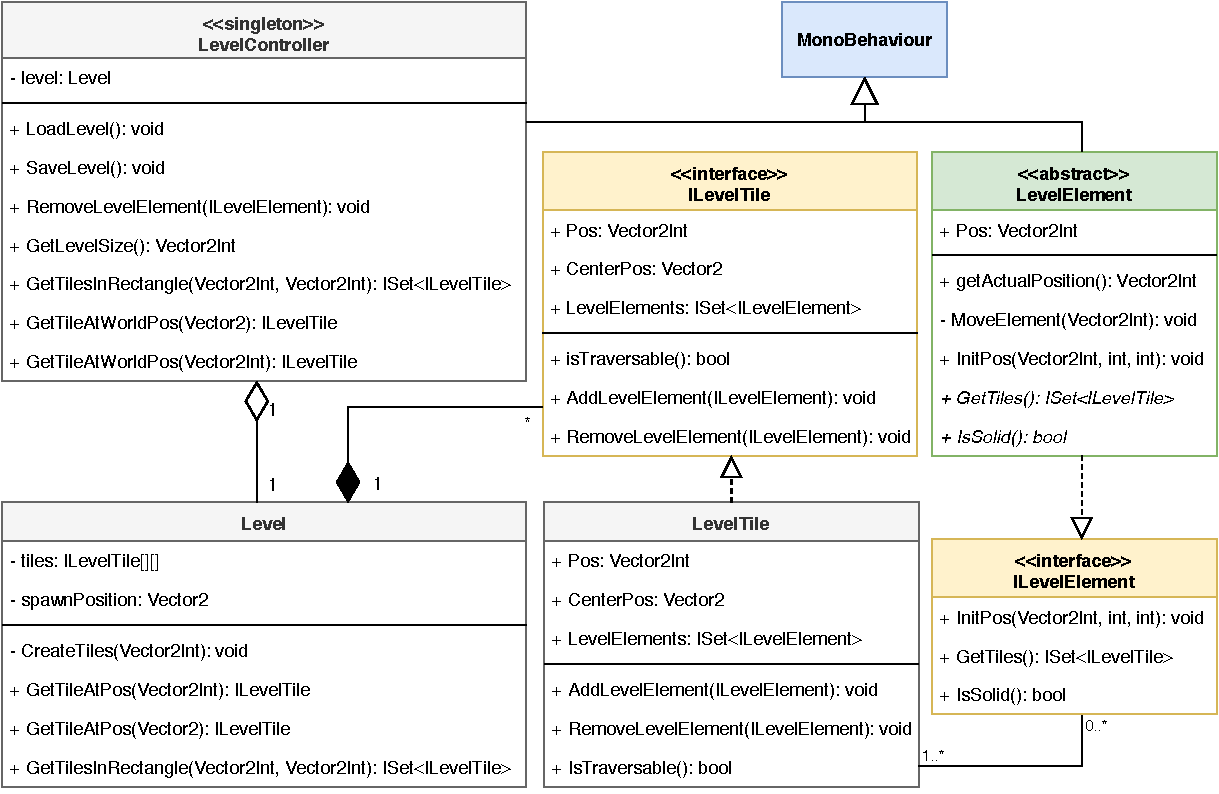
\includegraphics[width=1.0\linewidth]{diagrams/Level_Data_Structure.pdf}
 \captionof{figure}[Datenstruktur des Levels]{UML-Klassendiagramm der grundlegenden Levelstruktur in reduzierter Darstellung.}
	\label{fig:level_structure}
\end{figure}

Neben den einzelnen Levelteilen speichert das Level außerdem auch die Startposition des Spielers und bietet über diverse Methoden Zugriff auf die einzelnen Levelteile über Weltkoordinaten. Um die Level-Datenstruktur vor Manipulationen von außen zu schützen, übernimmt der \texttt{LevelController} die Verwaltung des Levels. Dieser existiert in der Unity-Szene für das eigentliche Spiel als einzelnes Spielobjekt und stellt alle notwendigen Operationen auf dem Level nach außen zur Verfügung. Der Controller hält außerdem eine Referenz auf die Datenstruktur des Levels und ist zuständig für das Speichern und Laden von Leveln. Wie dies konkret funktioniert, wird in Kapitel \ref{sec:designSerialization} im Zuge der Levelserialisierung und Deserialisierung genauer erläutert. Zusammenfassend bildet der \texttt{LevelController} also eine Zwischenschicht zwischen Zugriffen von außen und dem zugrundeliegendem Modell in Form des Levels.

Das Interface \texttt{ILevelTile}, aus dem sich das Level zusammensetzt, und welches die konkrete Klasse \texttt{LevelTile} implementiert, beinhaltet drei Eigenschaften:
\begin{itemize}
	\item \texttt{Pos}: Die linke untere Position des \texttt{ILevelTile} im Level.
	\item \texttt{CenterPos}: Die Koordinaten der Mitte des Teils. Diese Eigenschaft dient vor allem der Bequemlichkeit, um häufige Umrechnungen mit der tatsächlichen Position zu vermeiden.
	\item \texttt{LevelElements}: Alle Level-Elemente, die auf diesem Teil platziert sind.
\end{itemize}

Über die Methoden \texttt{AddLevelElement(...)} und \texttt{RemoveLevelElement(...)} können zur Laufzeit dynamisch Level-Elemente einem Teil zugeordnet und wieder entfernt werden. Die \texttt{Is\-Tra\-ver\-si\-ble()}-Methode dient dazu, zu ermitteln, ob zum Beispiel Gegner über dieses Teil laufen können und wird vor allem innerhalb des Wegfindesystems (siehe Kapitel \ref{sec:pathfindingConcept}) utilisiert. Die Entscheidung, ob ein \texttt{LevelTile} traversierbar ist, wird dabei basierend auf den darauf platzierten Level-Elementen getroffen.

Die \texttt{Level}-Klasse und die zugehörigen \texttt{ILevelTile} bieten soweit eine flexible Grundstruktur für das Level, jedoch fehlt noch eine Integration der tatsächlich in der Unity-Szene enthaltenen und für den Spieler sichtbaren Objekte in die beschriebene Datenstruktur. Diese Rolle übernehmen die bereits vorher erwähnten Level-Elemente. Ein solches Element ist konkret jeder beliebige statische Gegenstand der auf dem Level platziert werden kann, wie zum Beispiel eine Wand. Details zu den einzelnen implementierten Elementen folgen hierzu in Abschnitt \ref{sec:levelElements}. Alle Elemente müssen zumindest das \texttt{ILevelElement}-Interface implementieren. Mit Ausnahme von Böden erben alle anderen direkt von der abstrakten Klasse \texttt{LevelElement}, die bereits generische Logik implementiert. Die \texttt{LevelElement}-Klasse erbt wiederum von \texttt{MonoBehaviour}, wodurch es sich direkt als Komponente zu Spielobjekten in der Szene hinzufügen lässt.

Die \texttt{InitPos(...)}-Methode muss bei jedem Level-Element nach der Erzeugung mit der ge\-wünsch\-ten Position als Eingabe aufgerufen werden und registriert das Element anhand der Position und der Größe in X- und Y-Achsenrichtung bei den Levelteilen, auf denen es sich befindet und setzt die Position des zugehörigen Spielobjekts in der Welt entsprechend. Per Aufruf von \texttt{GetTiles()} lassen sich schließlich alle Levelteile, auf denen sich das Element befindet, zurückgeben. Dabei ist anzumerken, dass ein \texttt{LevelElement} keine direkte Referenz auf diese Levelteile hat, um eine zweiseitige Referenzierung zwischen den Teilen und Elementen zu vermeiden. Stattdessen nutzen die konkreten Implentierungen von \texttt{ILevelElement} die eigene Position und die Hilfsmethoden des \texttt{LevelController}, um auf die zugehörigen Teile zuzugreifen. Da die verschiedenen Levelelemente auch mehrere Teile groß sein und verschiedene Formen haben können, muss die \texttt{GetTiles()}-Methode von einer konkreten Unterklasse ausimplementiert werden, weil so das inhärente Wissen über die Form des Elements zur Ermittlung der zugeordneten Levelteile genutzt werden kann. Über den Aufruf von \texttt{IsSolid()} lässt sich schließlich noch ausgeben, ob ein Level-Element solide, also nicht begehbar ist. Dies wird deshalb über eine Methode anstatt einer einfachen boolschen Variable geregelt, weil sich der Rückgabewert zur Laufzeit ändern kann, wie zum Beispiel bei einer Tür, die verschlossen wird.

Über die Eigenschaft \texttt{Pos} lässt sich bei jedem abstrakten \texttt{LevelElement} außerdem die Position während des Spiels ändern. Die Methode \texttt{MoveElement(...)} bewegt dann automatisch das zugehörige Spielobjekt und aktualisiert die Referenzen der Levelteile auf dieses Level-Element, sodass diese mit der neuen Position übereinstimmen. \texttt{GetActualPosition()} gibt die tatsächlichen Weltkoordinaten des Spielobjekts des Level-Elements zurück.

Mit der beschriebenen Datenstruktur des Levels ist es also zusammenfassend möglich, Spielobjekte für die tatsächlichen Elemente des Levels flexibel auf dessen Raster zu platzieren und zu verschieben. Ebenso lassen sich alle für die Spiellogik relevanten Daten positionsbasiert durch die einzelnen Teile des Levels ermitteln.
 
\subsection{Die Level-Elemente des Spiels}\label{sec:levelElements}
Um ein Level mit sichtbaren Gegenständen populieren zu können, müssen noch die entsprechenden Level-Elemente implementiert werden. Wie die einzelnen Elemente, sowohl aus Sicht der damit verbundenen Logik, als auch in Bezug auf die grafische Darstellung umgesetzt sind, wird in den folgenden Abschnitten genau erläutert.

\begin{figure}[h]
 \centering
 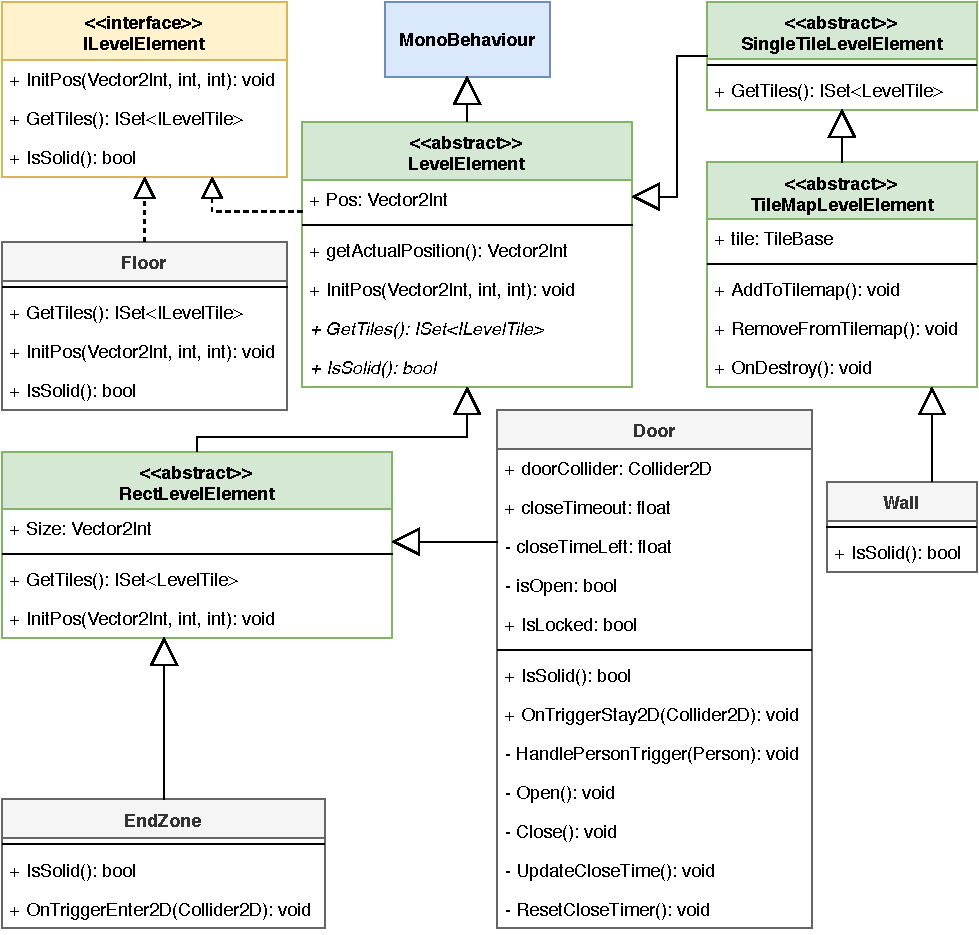
\includegraphics[width=0.86\linewidth]{diagrams/Level_Element_UML.pdf}
 \captionof{figure}[Übersicht über die Level-Elemente des Spiels]{UML-Klassendiagramm aller Level-Elemente des Spiels.}
	\label{fig:level_elements}
\end{figure}

Vor der konkreten Implementierung werden die Level-Elemente zunächst über die abstrakten Klassen \texttt{RectLevelElement} und \texttt{SingleTileLevelElement} weiter in größere rechteckige Elemente, und welche, die nur ein einzelnes Teil umfassen unterteilt, wie anhand des UML-Diagramms in Abbildung \ref{fig:level_elements} zu sehen ist. Beide implementieren die \texttt{GetTiles()}-Methode, da diese für jeweils alle Unterelemente gleich ist. Das \texttt{RectLevelElement} überschreibt zudem \texttt{InitPos(...)}, um bei der Initialisierung die Ausmaße des Elements in der entsprechenden Eigenschaft \texttt{Size} abzuspeichern. Der Nutzen des \texttt{TileMapLevelElement} wird im Folgeabschnitt \ref{sec:wall} am Beispiel der Wände im Level erklärt.

Allgemein wäre eine so feine Unterteilung durch die abstrakten Oberklassen in der aktuellen Form des Spiels noch nicht zwangsläufig notwendig gewesen. Unter dem Gesichtspunkt, dass zu einem späteren Zeitpunkt gegebenenfalls weitere Elemente hinzugefügt werden sollen, ist dies aber so mit einem nur sehr geringen Arbeitsaufwand möglich und daher dennoch sinnvoll.

\subsubsection{Wände}\label{sec:wall}
Wände sind die zentralen Bestandteile zur Aufteilung des Levels und sind genau ein Teil groß. Alle Spielobjekte, die eine Wand sind, besitzen zusätzlich einen quadratischen \textit{Collider2D}, sodass sie nicht durch den Spieler oder Gegner traversierbar sind.

Aus Sicht der Logik stellt dies bereits alles Relevante zu den Wänden dar, jedoch ergibt sich im Bezug auf die Grafik ein Problem. Sind mehrere Wände nebeneinander platziert, sollten sich die Texturen automatisch so anpassen, dass es so scheint als wären sie verbunden, wie in Abbildung exemplarisch \ref{fig:connected_walls} dargestellt ist.

\begin{figure}[h]
 \centering
 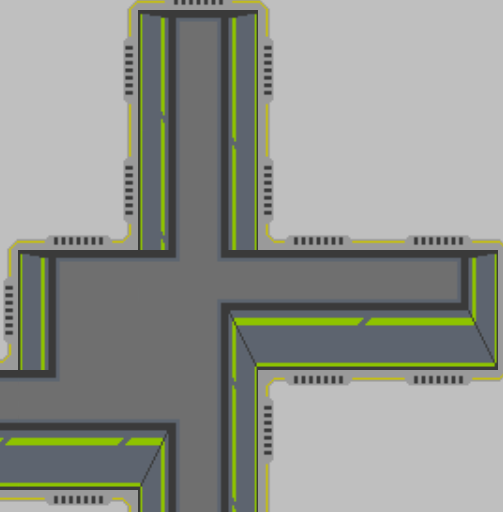
\includegraphics[width=0.3\linewidth]{pics/connected_walls.png}
 \captionof{figure}[Automatische Wandtexturverbindung]{Beispiel aus dem Spiel bei dem sich die Texturen mehrerer Wände automatisch verbinden. Bei den Bodenteilen ist selbiges zu sehen.}
	\label{fig:connected_walls}
\end{figure}

Mit einfachen Texturen auf den einzelnen Wandelementen wäre dies nur mit größerem Programmieraufwand zu lösen. Eine einfachere Lösung bietet hier die Verwendung einer sogenannte \textit{Tilemap} von Unity in Kombination mit \textit{RuleTiles}. Eine \textit{Tilemap} ist vereinfacht dargestellt ein Raster, bei dem jedem Feld des Rasters ein sogenanntes \textit{Tile} zugewiesen werden kann. Dies ist nicht zu verwechseln mit den Teilen in der Levelstruktur, denn die Teile der \textit{Tilemap} definieren lediglich eine grafische Repräsentation. Das \textit{RuleTile} ist dabei eine von Unity zur Verfügung gestellte Spezialform, die es ermöglicht zu definieren, bei welchen Nachbarschaftsbeziehungen welche Textur für das Teil geladen werden soll. Das heißt, es lässt sich beispielsweise für die Wände definieren, welches Bild für diese Wand angezeigt wird, wenn rechts davon ebenso eine Wand platziert ist. Dies ermöglicht, das vorher beschriebene Problem mit nur geringem Aufwand zu Lösen.

Konkret wird hierzu eine \textit{Tilemap} für Wände angelegt, die sich in der Rastergröße mit der des Levels überlagert, sodass die Teile über der tatsächlichen Position des Levels angezeigt werden. Für solche \textit{Tilemap}-basierte Level-Elemente wird zusätzlich die abstrakte Oberklasse \texttt{TileMapLevelElement} angelegt, von der die Wand erbt. Diese hält eine Referenz auf die Vorlage für das \textit{Tile} und besitzt die Funktionalität, in der \textit{Tilemap} das \textit{Tile} an der entsprechenden Position auf die Vorlage (hier die Wand) zu setzten, beziehungsweise diese wieder zu entfernen. Bei Zerstörung des Spielobjekts der Wand wird das entsprechende \textit{Tile} auf der \textit{Tilemap} automatisch wieder entfernt.

Die Wand ist somit aufgeteilt in das Spielobjekt, welches für die eigentliche Logik verantwortlich ist, sowie die grafische Repräsentation auf der \textit{Tilemap}.

\subsubsection{Böden}\label{sec:floor}
Böden stellen unter den Level-Elementen eine Ausnahme dar, weil sie als einzige nicht von \texttt{LevelElement} erben sondern direkt das \texttt{ILevelElement}-Interface implementieren. Sie sind ebenso wie Wände ein Teil groß und verwenden zur Anzeige auch eine eigene \textit{Tilemap}, sodass die Texturen benachbarter Böden sich verbinden können. Auf den ersten Blick wäre es daher logisch, wenn die Klasse \texttt{Floor} von \texttt{TileMapLevelElement} erben würde. Tatsächlich wäre dies die aus softwarearchitektonischer Sicht gesehen bessere Lösung, da die \texttt{Tilemap}-bezogene Logik komplett wiederverwendet werden könnte.

Der Grund warum sich dagegen entschieden wurde ist, dass Böden an sich keine Logik im Spiel besitzen und der rein dekorativen, grafischen Anzeige dienen. Alle \texttt{LevelElemente} sind aber aufgrund der \textit{MonoBehaviour}-Oberklasse an ein Spielobjekt gebunden. Das bedeutet, dass für jeden Boden ein Spielobjekt angelegt werden würde, was de-facto in der Szene ohne Nutzen ist, weil keine Logik an ein Bodenteil gebunden ist. Es würde also unnötigerweise Arbeitsspeicher und Rechenzeit für die Spielobjekte der Böden verbraucht werden. Deshalb implementieren diese nur das entsprechende Interface für Level-Elemente und existieren so nur innerhalb der Datenstruktur des Levels und als grafisches \textit{Tile} in der entsprechenden \textit{Tilemap}. Das setzen des \textit{Tiles} erfolgt dabei unmittelbar nach der Erzeugung eines Boden-Objekts.

\subsubsection{Türen}\label{sec:door}
Die Türen sind in Bezug auf die damit verbundene Spiellogik die komplexesten Level-Elemente, was in Abbildung \ref{fig:level_elements} bereits zu erkennen ist. Es handelt sich dabei um ein \texttt{RectLevelElement}, da diese je nach Rotation zwei Teile breit sind. Der Spielausschnitt in Abbildung \ref{fig:door_opening} zeigt, wie sich die Tür automatisch bei Annäherung eines Spielers oder Gegners öffnen soll.

\begin{figure}[h]
 \centering
 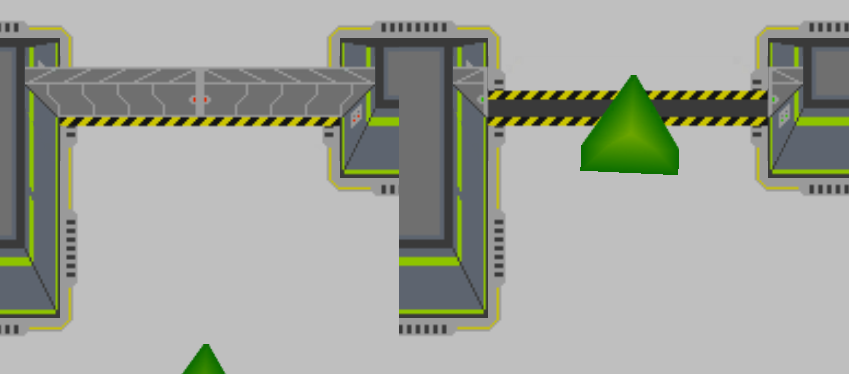
\includegraphics[width=0.6\linewidth]{pics/traversing_door.png}
 \captionof{figure}[Automatischen öffnen einer Tür]{Automatisches Öfnen einer Tür bei Annäherung einer Person.}
	\label{fig:door_opening}
\end{figure}

Um dieses Verhalten zu realisieren, werden zwei verschiedene rechteckige \textit{Collider2D} eingesetzt. Einer ist deutlich größer als die Tür und ist als sogenannter \textit{Trigger} gesetzt. Das bedeutet, dass bei Kontakt mit einem anderen physikalischen Objekt von der Physik-Engine entsprechende Methoden, wie hier \texttt{OnTriggerStay2D(...)}, aufgerufen werden, aber keine tatsächlichen Kollisionen simuliert werden. Der Spieler prallt also beispielsweise nicht von diesem \textit{Collider2D} ab. Befindet sich eine Person in diesem Bereich, wird die Tür geöffnet und die Zeit bis die Tür wieder geschlossen wird zurückgesetzt. Befindet sich keine Person mehr in diesem \textit{Trigger}-\textit{Collider2D}, schließt sich die Tür nach Ablauf des \texttt{closeTimeout} wieder.

Die Tür hält zudem eine Referenz auf einen weiteren \textit{Collider2D}, der so groß wie die Tür an sich ist. Im Gegensatz zu ersterem verursacht dieser Kollisionen, sodass bei geschlossener Tür zum Beispiel Schüsse daran aufprallen. Wird die Tür geöffnet, wird dieser dann vorübergehend deaktiviert. Die Eigenschaft \texttt{IsLocked} ermöglicht außerdem die Tür zu versperren, wodurch sie sich nicht mehr automatisch bei Annäherung einer Person öffnet. Diese Funktionalität wird zwar im aktuellen Stand nicht verwendet, eröffnet aber Möglichkeiten für zukünftige Erweiterungen.

Für das Öffnen und Schließen der Tür existieren zudem entsprechende Animationen. Die Zustandsübergänge des zugehörigen \textit{Animators} wurden bereits beispielhaft in Abbildung \ref{fig:animator_example} dargestellt.

\subsubsection{Endzone}\label{sec:endZone}
In diesem Spiel soll es dem Spieler nicht nur möglich sein durch Eliminierung aller Gegner zu gewinnen. Stattdessen soll es ebenso ermöglicht werden den Sieg durch Erreichen einer Level-Endzone zu erringen, indem die Gegner geschickt aus­ma­nö­v­rie­rt werden. Dadurch soll auch leises Vorgehen seitens des Spielers belohnt werden.

Diese Endzone muss allerdings noch in das Spiel integriert werden. Hierzu wird ein weiteres \texttt{RectLevelElement} namens \texttt{EndZone} erstellt. Das zugehörige Spielobjekt enthält neben der Textur, ähnlich wie die Tür, einen als \textit{Trigger} dienenden \textit{Collider2D}. Sobald ein physikalisches Objekt mit diesem eine Kollision auslöst, wird die \texttt{OnTriggerEnter2D(...)}-Methode aufgerufen. Handelt es sich bei dem kollidierenden Objekt um den Spieler, gilt das Spiel als gewonnen und das Menü zum Spielende öffnet sich. Von dort aus kann der Nutzer das Level entweder neu starten, oder in das Hauptmenü zurückkehren.